%\documentclass{beamer}
%\documentclass[c]{beamer}
 \documentclass[t]{beamer}
%\documentclass[b]{beamer}
\listfiles
\usepackage{tikz}
\usetikzlibrary{positioning}
\usetikzlibrary{decorations.text}
\usetikzlibrary{decorations.pathmorphing}
\usetikzlibrary{fit}
\usetikzlibrary{shapes}

\mode<presentation>
{
  \usetheme[english]{KIT}
% \usetheme[usefoot]{KIT}
% \usetheme[deutsch]{KIT}

%%  \usefonttheme{structurebold}

  %\setbeamercovered{transparent}
  \setbeamercovered{invisible}

  %\setbeamertemplate{enumerate items}[circle]
  \setbeamertemplate{enumerate items}[ball]
}

\usepackage{babel}
\date{29.10.13}
%\DateText

%\KITfoot{\parbox[t]{90mm}{\today:\qquad Dies ist eine sehr lange selbstdefinierte Fu\ss{}zeile -- Dies ist eine sehr lange selbstdefinierte Fu\ss{}zeile -- Dies ist eine sehr lange selbstdefinierte Fu\ss{}zeile}}


\usepackage[utf8]{inputenc}
\usepackage[T1]{fontenc}
\usepackage{array}
\usepackage{minted}

\usenavigationsymbols
%\usenavigationsymbols[sfHhdb]
%\usenavigationsymbols[sfhHb]



\begin{document}





\begin{frame}[fragile]
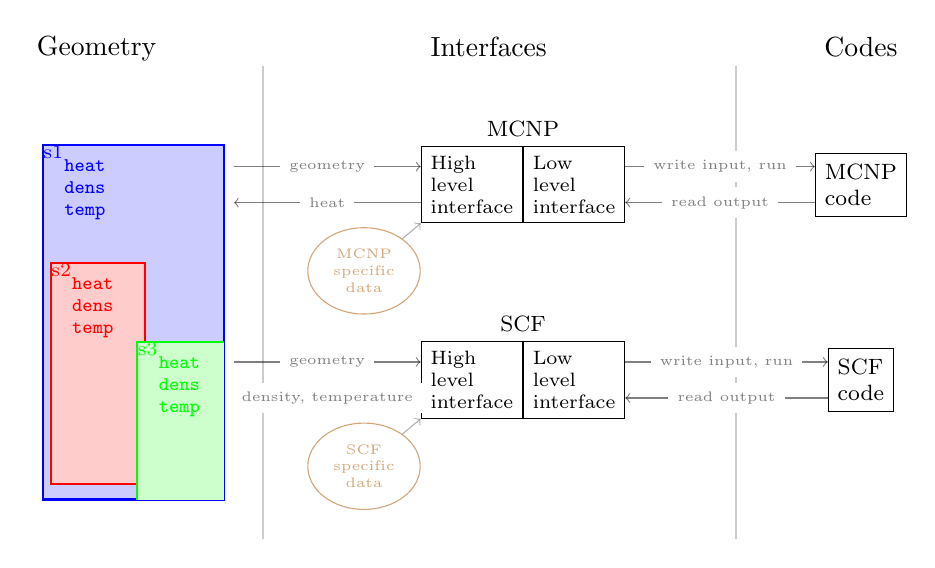
\begin{tikzpicture}
    %\draw[help lines, thin, color=blue!10] (0,0) grid (11,7);
    \tikzstyle{every node}=[font=\footnotesize]%, draw=black!10]%, draw=black, rounded corners, text centered]%, minimum height=1cm, text width=4cm]
    % Titles
    \tikzstyle{Titles}=[font=\normalsize, anchor=north west]
    \node[Titles] at (0,7) (t1) {Geometry};
    \node[Titles] at (5,7) (t2) {Interfaces};
    \node[Titles] at (10,7) (t3) {Codes};

    % vertical delimiters
    \tikzstyle{DelimiterLines}=[color=black!20, thick]
    \draw[DelimiterLines] (3, 6.5) -- +(0,-6cm);
    \draw[DelimiterLines] (9, 6.5) -- +(0,-6cm);

    % model example
    \coordinate (m1) at (0.2, 1);
    \coordinate (m2) at (2.5, 5.5);
    \coordinate (m3) at (0.3, 1.2);
    \coordinate (m4) at (1.5, 4.0);
    \coordinate (m5) at (1.4, -1);
    \coordinate (m6) at (2.7, 3.0);
    \node[opacity=0., fit=(m1) (m2)] (model) {};
    \begin{scope}% scope here while clipping.
        \path[clip] 
            [preaction = {draw=blue,thick, fill=blue!20}]
            (m1) rectangle (m2);
        \path[thick, fill=red!20,   draw=red]   (m3) rectangle (m4);
        \path[thick, fill=green!20, draw=green] (m5) rectangle (m6);
    \end{scope}
    
    \tikzstyle{SolidLabels}=[align=right,font=\scriptsize, opacity=0., text opacity=1., inner sep=0., anchor=north west]
    \tikzstyle{MeshLabels}=[SolidLabels,font=\scriptsize\tt]
    \node[SolidLabels, text=blue] at (m1 |- m2) (s1) {s1};
    \node[SolidLabels, text=red]   at (m3 |- m4) (s2) {s2};
    \node[SolidLabels, text=green] at (m5 |- m6) (s3) {s3};

    \node[MeshLabels,  text=blue,  below right=0mm of s1] (m1) {heat\\dens\\temp};
    \node[MeshLabels,  text=red,   below right=0mm of s2] (m2) {heat\\dens\\temp};
    \node[MeshLabels,  text=green, below right=0mm of s3] (m3) {heat\\dens\\temp};

    % % interfaces
    \tikzstyle{Interfaces}=[draw=black,rectangle split, rectangle split parts=2, rectangle split horizontal=true, minimum height=0.8cm, align=left,font=\scriptsize]
    \tikzstyle{SpecData}=[color=brown, draw, ellipse, align=center, font=\tiny, opacity=0.7]

    \node[Interfaces, anchor=west, label=above:MCNP] at (5, 5) (mi) {High\\level\\interface \nodepart{second} Low\\level\\interface};
    \node[SpecData, below left=3mm of mi] (msd) {MCNP\\specific\\data};

    \node[Interfaces, below=15mm of mi, label=above:SCF] (si) {High\\level\\interface \nodepart{second} Low\\level\\interface};
    \node[SpecData, below left=3mm of si] (ssd) {SCF\\specific\\data};



    % codes
    \tikzstyle{Codes}=[draw=black, minimum height=0.8cm, align=left]
    \node[Codes, align=left] at (t3 |- mi) (mcnp) {MCNP\\code};
    \node[Codes, align=left] at (t3 |- si) (scf)  {SCF\\code};


    %% connections
    \tikzstyle{ConnectionNodes}=[font=\tiny, fill=white, fill opacity=1., text opacity=0.5, align=center]
    \tikzstyle{ConnectionLines}=[opacity=0.5]

    % model -- MCNP interface
    \draw[ConnectionLines, ->] (model.east |- mi.170) -- node[ConnectionNodes] {geometry} (mi.170);
    \draw[ConnectionLines, <-] (model.east |- mi.190) -- node[ConnectionNodes] {heat}     (mi.190);

    % MCNP interface -- MCNP
    \draw[ConnectionLines, ->] (mi.10)  -- node[ConnectionNodes] {write input, run} (mcnp.west |- mi.10);
    \draw[ConnectionLines, <-] (mi.-10) -- node[ConnectionNodes] {read output}      (mcnp.west |- mi.-10);

    % model -- SCF interface
    \draw[ConnectionLines, ->] (model.east |- si.170) -- node[ConnectionNodes] {geometry}             (si.170);
    \draw[ConnectionLines, <-] (model.east |- si.190) -- node[ConnectionNodes] {density, temperature} (si.190);

    % SCF interface -- SCF
    \draw[ConnectionLines, ->] (si.10)  -- node[ConnectionNodes] {write input, run} (scf.west |- si.10);
    \draw[ConnectionLines, <-] (si.-10) -- node[ConnectionNodes] {read output}      (scf.west |- si.-10);

    % code specific data
    \draw[ConnectionLines, ->, opacity=0.3] (msd) -- (mi.south west);
    \draw[ConnectionLines, ->, opacity=0.3] (ssd) -- (si.south west);



\end{tikzpicture}

\end{frame}




\end{document}
